\chapter{Trabalhos Relacionados}\label{cap_exemplos}

A presente pesquisa foi realizada a partir do levantamento de informações sobre os principais sistemas gerenciadores de conteúdo do mercado. Pretende-se classificá-los a partir de sua quota de mercado, popularidade e características semelhantes aos requisitos necessários ao Painel Pró-Mamá. Por fim, serão selecionados três, de acordo com alguns critérios, para um detalhamento a fim de elucidar as principais funcionalidades, vantagens/desvantagens e sua portabilidade para construção de um painel administrativo.

\section{Pesquisa de mercado}

Foi utilizado como base a pesquisa realizada pela \citeonline{w3techs_cms}, uma organização responsável por monitorar e analisar diversas tecnologias na internet. Em seus estudos buscou-se a análise da presença de mercado dos CMS na publicação de websites. No gráfico abaixo pode-se analisar duas barras, em vermelho representam sites criados com sistema gerenciador de conteúdo e em azul sites com dados estáticos.

\begin{figure}[htb]
  \caption{\label{fig_grafico} Quota de mercado dos CMS}
  \begin{center}
    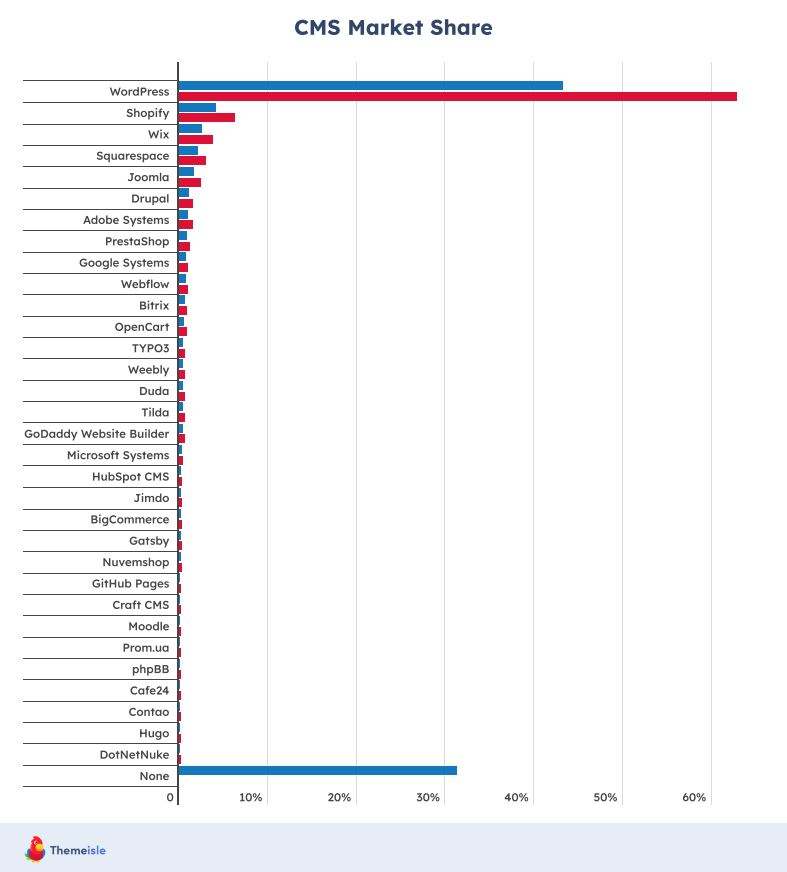
\includegraphics[scale=0.45]{imagens/w3techs-cms.JPG}
  \end{center}
  \legend{Fonte: \citeonline{themeisle_cms_market_share}}
\end{figure}

Atualmente cerca de 69\% dos sites na internet foram criados a partir de um CMS, dessa parcela, somente o WordPress detém de aproximadamente 43\% de todos os websites. Apesar da predominância do WordPress, destacam-se também a plataforma Wix e Shopify que vem logo em seguida no ranking.

\section{Detalhamento}

Dado os CMS mencionados, serão traçadas informações e detalhes a seu respeito nesta seção.

\subsection{WordPress}

O \citeonline{wordpress} é uma plataforma CMS de código aberto utilizada na criação de cerca de 43\% de todos os websites presentes na internet. Sua configuração em muitos serviços de hospedagem, como a HostGator, pode ser solicitada em conjunto com o plano selecionado, bastando apenas alterar seu domínio para redirecionar para o servidor. No caso da instalação manual é preciso atender aos requisitos: PHP v7.4 ou superior, MySQL v5.7 / MariaDB v10.3 ou superior e suporte HTTPS, para assim transferir via FTP o sistema e instalá–lo em conjunto com a base de dados.

Uma de suas principais vantagens é o painel de edição que permite com que sejam construídas interfaces a partir de temas disponibilizados pela comunidade. Nesta seção de aparência há dois temas iniciais, porém também encontra-se um repositório com milhares, alguns pagos e outros gratuitos. Apesar de ser um software livre, o intuito do produto é que sejam comercializados plugins para que o dono do site consiga adicionar as funcionalidades desejadas.

No mesmo local do editor outros usuários podem acessar para gerenciar o conteúdo do site, assim o WordPress permite com que sejam designados papéis para controle de quem pode editar a estrutura ou somente o texto de espaços pré-definidos por outro administrador.

Além de acessar por navegador web, o WordPress possui seu aplicativo disponível nas lojas para que o administrador possa gerenciar seu site a partir de seu dispositivo móvel.

\subsection{Wix}

\citeonline{wix} é a plataforma paga para criação e gerenciamento de conteúdo de sites que mais se popularizou nos últimos tempos, seguida de WordPress e Shopify. Sua quota de mercado cresceu em torno de 800\% entre 2016 e 2023. Criada em 2006, seu objetivo é simplificar a publicação de websites sem a necessidade de conhecimento prévio.

Não há necessidade de instalar ou contratar um serviço de hospedagem, basta conectar seu domínio e configurar um tema para que já se possa visualizar o site em construção. Seus templates vão desde: blog, landing page, portfólio, marketplace, anúncios, etc.

Uma de suas principais funcionalidades é o editor com tecnologia arrasta e solta, a qual permite com que o administrador mova os elementos do site da maneira que quiser. Cada elemento de design é personalizável, sendo possível redimensionar, recolorir, girar e alinhar até atingir a forma desejada.

Outra aposta está em sua ferramenta de inteligência artificial Wix ADI, onde algumas perguntas são feitas e a partir delas um site com conteúdo e imagens integradas é criado. Durante as etapas é possível personalizar a paleta de cores, logo, design e assim o restante é construído de forma personalizada as regras de negócios identificadas pelo usuário.

Assim como o WordPress, o aplicativo Wix Owner também é designado para gerenciar o site, possui funcionalidades como: edição e compartilhamento de posts, aceitação de reservas e pagamentos, conversa pelo chat com visitantes, etc. A ideia é que o dono do site possa acessar seu portal tanto a partir do navegador web, quanto pelo seu dispositivo móvel.

\subsection{Shopify}

\citeonline{shopify} é uma plataforma de e-commerce lançada em 2006 que permite a indivíduos e empresas criarem suas próprias lojas onlines. Atrás somente do WordPress, é o segundo CMS mais popular do mercado, só nos Estados Unidos são mais de dois milhões e meio de comércios eletrônicos publicados.

Assim como o Wix, não é necessário instalá-lo, uma vez conectado ao domínio é possível visualizar a loja na internet. Como um sistema líder na temática de varejo, seus templates seguem os modelos de lojas virtuais, com listagem de produtos e páginas de checkout. Há também a possibilidade de criar blogs pessoais e landing pages, porém qualquer personalização que vá além deve ser feita manualmente pelo editor.

Por tratar de marketplaces, sua infraestrutura é robusta e confiável, o que garante boa velocidade de carregamento das páginas e alta confiabilidade. Além de suporte 24/7 via chat em qualquer plano contratado.

Seus recursos se assemelham aos plugins do WordPress, nesse caso na loja aplicativos podem ser configurados para adicionar as funcionalidades, há desde: gestão de inventário, análise de dados, marketing, gateway de pagamentos, tudo que um comércio precisa.

\section{Comparações}

Dentre os sistemas analisados, dado que seu uso é genérico, ou seja, são ferramentas que permitem a criação de: blogs, comércios digitais, landing page, etc. Será comparado a partir do viés de sua utilização em painéis administrativos e como o conteúdo é distribuído para não só o site na web, mas sim para dispositivos móveis. Por isso, os três CMS possuem uma condição inicial em comum que é a possibilidade de acesso do dado via API Rest, assim a aplicação móvel pode fazer solicitações HTTP para consumir e atuar em cima das entidades.

Algumas tabelas serão apresentadas para que sejam vistos os comparativos produzidos:

\begin{table}[htb]
  \begin{center}
    \ABNTEXfontereduzida
    \caption{comparações entre os sistemas selecionados.}
    \label{tab-comparacao-1}
    \begin{tabular}{c|c|c|c}
      %\hline
      \phantom{.}     & \textbf{Tema administrativo} & \textbf{Design responsivo} & \textbf{Gratuito} \\
      \hline
      WordPress       & X                            & X                          &
      X                                                                                               \\
      \hline
      Wix             & \phantom{.}                  &
      X               & \phantom{.}                                                                   \\
      \hline
      Shopify         & \phantom{.}                  & X                          & \phantom{.}       \\
      \hline
      Painel Pró-Mamá & X                            & X                          & X                 \\
      % \hline
    \end{tabular}
    \legend{Fonte: autor.}
  \end{center}
\end{table}

Conforme as informações acima da \autoref{tab-comparacao-1}, pode-se observar que além do WordPress que é líder de mercado, apenas o Painel Pró-Mamá oferece tema administrativo de forma gratuita e com estilização responsiva.

\begin{table}[htb]
  \begin{center}
    \ABNTEXfontereduzida
    \caption{comparações entre os sistemas selecionados.}
    \label{tab-comparacao-2}
    \begin{tabular}{c|c|c}
      %\hline
      \phantom{.}     & \textbf{Enviar e-mail} & \textbf{\emph{Push notification}} \\
      \hline
      WordPress       & X                      & X*                                \\
      \hline
      Wix             & X                      &
      X*                                                                           \\
      \hline
      Shopify         & X                      & \phantom{.}                       \\
      \hline
      Painel Pró-Mamá & X                      & X                                 \\
      % \hline
    \end{tabular}
    \legend{Fonte: autor.}
  \end{center}
\end{table}

A partir da \autoref{tab-comparacao-2}, como a maioria das ferramentas de mercado, todas implementam o envio de e-mail para seus usuários. Porém, somente WordPress e Wix tem em suas lojas plugins para Push Notification, entretanto este somente funciona para o site web, ao contrário do que o Painel Pró-Mamá oferece que é o envio da notificação para os usuários do aplicativo nos dispositivos móveis.

\begin{table}[htb]
  \begin{center}
    \ABNTEXfontereduzida
    \caption{comparações entre os sistemas selecionados.}
    \label{tab-comparacao-3}
    \begin{tabularx}{\textwidth}{|c|>{\centering\arraybackslash}X|>{\centering\arraybackslash}X|>{\centering\arraybackslash}X|>{\centering\arraybackslash}X|>{\centering\arraybackslash}X|}
      %\hline
      \phantom{.}     & \textbf{Facilidade uso usuário não técnico} & \textbf{Gráfico e estatísticas} & \textbf{CRUD de dados} & \textbf{Envio de arquivos} & \textbf{Exportação de dados em diferentes formatos} \\
      \hline
      WordPress       & \phantom{.}                                 & X                               &
      X               & X                                           & \phantom{.}                                                                                                                                 \\
      \hline
      Wix             & X                                           &
      X               & X                                           & X                               & \phantom{.}                                                                                               \\
      \hline
      Shopify         & X                                           & X                               & X                      & X                          & \phantom{.}                                         \\
      \hline
      Painel Pró-Mamá & X                                           & X                               & X                      & X                          & X                                                   \\
      % \hline
    \end{tabularx}
    \legend{Fonte: autor.}
  \end{center}
\end{table}

Observa-se na \autoref{tab-comparacao-3} que assim como todos os CMS, o Painel Pró-Mamá também possibilita a manipulação e visualização dos dados, sendo texto ou arquivo. Porém dentre os sistemas gratuitos, é o único que se preocupa com o uso por usuário não técnico, haja vista que tratam-se dos servidores públicos do projeto Pró-Mamá.

Outro ponto interessante do Painel Pró-Mamá é a capacidade de exportar os dados nos formatos auxiliares a sistemas da secretaria de saúde do município de Osório, facilitando assim o cadastro das mães pelos profissionais responsáveis.
